\documentclass[../defence.tex]{subfiles}
\begin{document}

  \begin{frame}{Landauniveaus I}
    \pause
    \begin{itemize}
      \item Energiequantelung von Ladungsträgern im Magnetfeld
      \pause
      \item Bewegung orthogonal zum Magnetfeld auf Kreisbahnen
      \pause
      \item Quantisierte Kreisbahnen wegen quantisiertem Spin
    \end{itemize}
    \pause
    \begin{equation*}
        E_n^\mathrm{Landau}=\left( n+\frac{1}{2}\right)\hbar\omega_\mathrm{c}+\frac{\hbar^2k_z^2}{2m}
    \end{equation*}
    \pause
    \begin{columns}[onlytextwidth, T]
      \column{\dimexpr\linewidth / 20 * 10}
        \begin{equation*}
          \omega_c = \frac{eB}{m}
        \end{equation*}
      \column{\dimexpr\linewidth / 20 * 9}
        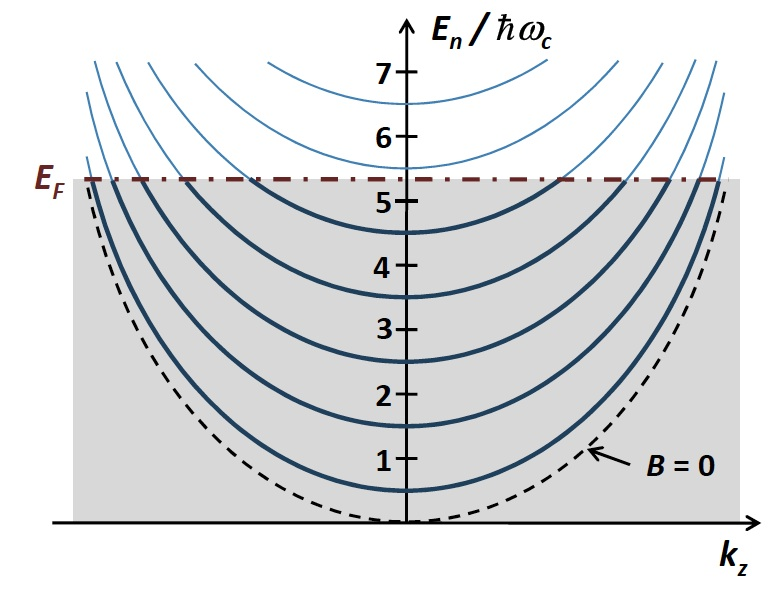
\includegraphics[width=\linewidth]{images/landau_parabeln.png}
      \column{\dimexpr\linewidth / 20}
        \cite{gross}
    \end{columns}
  \end{frame}
  \note{
  \begin{itemize}
    \item Landau Niveaus $\rightarrow$ Energiequantelung von Ladungsträgern im Magnetfeld
    \item Bewegung orthogonal zum Magnetfeld auf quantisierten Kreisbahnen
    \item Kreisbahnen quantisiert wegen quantisiertem Spin
    \item Plot der Energien
  \end{itemize}
  }

\end{document}
